\section{度量熵与次高斯过程}

对于次高斯

%ε网、ε包、ε覆盖、均匀离散集、相对密集集和德尔尼集(以鲍里斯·德尔尼命名)是几个紧密相关的定义,用于描述点集的良好分布,这些集合的包络半径和覆盖半径衡量了它们的分布情况。
%这些集合在编码、近似算法等理论中有着应用. 

\subsection{覆盖数、填装数与度量熵}

在度量空间理论中, $\delta$-网,  $\delta$-覆盖, $\delta$-填装是几个紧密相关的定义,可以用于描述点集的良好分布. 

集合$\cT \subseteq \cX$关于度量$\rho$的一个\textbf{$\delta$-覆盖}是指$\cT$的子集$\{\theta^1, \dots, \theta^N\}$满足对任意$\theta \in \cT$, 都存在某个$\theta^i$使得$\rho(\theta, \theta^i) \leq \delta$. 
\textbf{$\delta$-覆盖数}$N(\delta; \cT, \rho)$是最小的$\delta$-覆盖的基数. 
我们称$\cT$\textbf{完全有界}的, 如果对任意$\delta > 0$, $N(\delta; \cT, \rho)$总是有限的. 
我们总是考虑完全有界的集合. 

集合$\cT \subseteq \cX$关于度量$\rho$的一个\textbf{$\delta$-填装}是指$\cT$的子集$\{\theta^1, \dots, \theta^N\}$, 满足对任意不同的$i, j \in \{1, \dots, N\}$, 都有$\rho(\theta^i, \theta^j) > \delta$——$\delta$-填装可以看作是半径为$\delta/2$、互不相交的球心的集合. 
\textbf{$\delta$-填装数}$N(\delta; \cT, \rho)$是最大的$\delta$-覆盖的基数. 

\begin{figure}[H]
	\centering 
	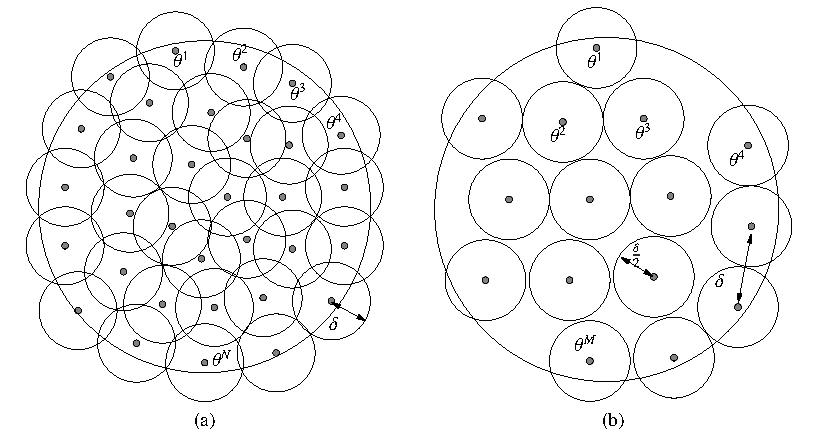
\includegraphics[width=.95\textwidth]{figure/covering-packing.pdf}
\end{figure}


在几何上, 覆盖数和填装数分别是覆盖集合所需最少的球的个数和集合最多填装的球的个数. 
尽管并不相同, 但是他们都描述了点集的良好分布——即不要相具太远、也不要过于拥挤——如此稀疏有致的点集. 

\begin{lemma}[覆盖数和填装数]\label{lemma:CoveringAndPacking}
	对所有$\delta > 0$, 覆盖数和填装数有如下关系
	\begin{equation*}
		M(2 \delta; \cT, \rho)
		\leq N(\delta; \cT, \rho)
		\leq M(\delta; \cT, \rho). 
	\end{equation*}
\end{lemma}


容易看到覆盖数关于$\delta$是非增的, 并且在$\delta \downarrow 0$时, 覆盖数通常是发散的. 
我们关注$\log N(\delta; \cT, \rho)$发散的速度, 这被称为$\cT$关于$\rho$的\textbf{度量熵}. 

尽管我们它成为“熵”, 度量熵是一个完全非随机、纯粹是几何的概念. 
下面的引理将度量熵和体积比联系起来, 其中涉及了Minkowski和的概念. 
\begin{lemma}
	设$\mathbb{B}$和$\mathbb{B}'$分别为$\R^d$中两种范数$\|\cdot\|$和$\|\cdot\|'$下的单位球, 那么在$\|\cdot\|$范数下, $\mathbb{B}'$的$\delta$-覆盖数满足界
	\begin{equation*}
		\delta^{-d} \frac{\vol(\mathbb{B}')}{\vol(\mathbb{B})}
		\leq N(\delta; \mathbb{B}', \|\cdot\|) 
		\leq \frac{\vol\left(\frac{2}{\delta} \mathbb{B}' + \mathbb{B} \right)}{\vol(\mathbb{B})}. 
	\end{equation*}
\end{lemma}
\begin{proof}
	若$\{\theta^1, \cdots, \theta^N\}$为$\mathbb{B}'$的一个$\|\cdot\|$范数下的$\delta$-覆盖, 即有$\mathbb{B}' \subseteq \cup_j \{\theta^j + \delta \mathbb{B}\}$, 于是$\vol(\mathbb{B}') \leq N \vol(\delta \mathbb{B}) = N \delta^d \vol(\mathbb{B})$, 从而得到左侧不等式. 
	
	另一方面, 令$\{\theta^1, \cdots, \theta^M\}$为$\mathbb{B}'$的一个$\|\cdot\|$范数下最大的$\delta/2$-填装, 这样的集合一定是$\mathbb{B}'$的一个$\|\cdot\|$范数下的$\delta$-覆盖. 
	于是球集$\{\theta^j + \delta/2 \cdot \mathbb{B} \}$中元素两两不交且包含在球$\mathbb{B}' + \delta/2 \cdot \mathbb{B}$中, 从而有$M \vol(\delta/2 \cdot \mathbb{B}) \leq \vol(\mathbb{B}' + \delta/2 \cdot \mathbb{B})$, 由此得到右侧不等式. 
\end{proof}

特别地, 如果我们取两种相同的范数, 可以得到单位球度量熵的上下界
\begin{equation*}
	d \log \frac{1}{\delta}  
	\leq \log N(\delta; \mathbb{B}, \|\cdot\|) 
	\leq d \log \left(1 + \frac{2}{\delta}\right). 
\end{equation*}
于是欧氏空间中, 单位球至多可以被$(1+2/\delta)^d$个半径为$\delta$的球覆盖. 
此外, $d$维立方体$[-1,1]^d$是范数$\|\cdot\|_{\infty}$下的单位球$\mathbb{B}^d_{\infty}$, 从而度量熵的阶为$d \log(1+1/\delta)$. 


\begin{example}[一个函数类的度量熵]
	考虑含参函数类
	\begin{equation*}
		\mathscr{F} := \{f_{\theta}(x) = 1 - e^{-\theta x} \colon x \in [0,1],\; \theta \in [0,1] \}
	\end{equation*}
	关于一致范数$\|\cdot\|_{\infty}$下的度量熵. 
	
	
\end{example}












